\section{Spannungsversorgung}\label{sec.spannungsversorgung}
In diesem Abschnitt soll auf die hardwareseitige Umsetzung der Spannungsversorgung für die Wetterstation eingegangen werden. Ziel ist der Entwurf einer Platine, auf der sämtliche Anforderungen umgesetzt werden.

\subsection{Anforderungen}\label{subsec.anforderungen}
Zunächst sollen in diesem Abschnitt die Anforderungen, die sich aus der Aufgabenstellung ableiten lassen, sowie solche, die sich aus den weiteren Überlegungen zur Umsetzung der Wetterstation ergeben.

\begin{itemize}

	\item Messung des Ladestroms
	\item Messung der Batteriespannung (Ladezustand)
	\item Messung des Stromverbrauchs der Wetterstation

\end{itemize}

Des Weiteren soll der Stromverbrauch der Wetterstation so niedrig wie möglich sein, um die Puffer-Batterie zu schonen und sonnenarme Phasen bzw. die Nacht ohne Stromausfall überbrücken zu können. Die verwendete Batterie hat eine Ladeschlussspannung von 12\,V. Da für den Mikrocontroller und die Sensoren allerdings Spannungspegel von 3,3\,V und 5\,V benötigt werden, müssen diese auf der Platine erzeugt werden.

Aus den mechanischen Anforderungen, dass Mikrocontroller, Platine und Sensoren möglichst in einem Gehäuse untergebracht werden sollen, ergibt sich, dass die entworfene Platine auf die Pinheader des Mikrocontrollers gesteckt werden soll. Auf Grund des Umfangs werden zwei Platinen Layoutet: Ein Powerboard zur Erzeugung der benötigten Spannungen und ein Sensor-Board, auf dem sich der Schaltungsteil für die Sensoren befindet.

\subsection{Power-Board}
In Abbildung \ref{fig.powerboard} wird das finale Layout des Power-Boards gezeigt. Im folgenden sollen einige wichtige Details des Stromlaufplans dargestellt.

\begin{figure}[H]
  \centering
  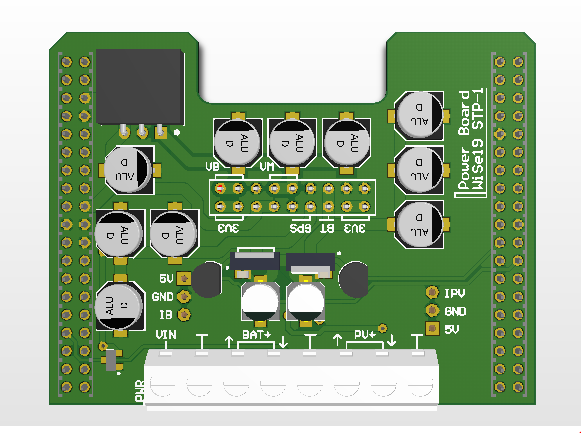
\includegraphics[width=0.7\textwidth]{./img/PCB_Power_3D_top.png}
  \caption{Power-Board}\label{fig.powerboard}
\end{figure}

Wesentliche Komponenten des Power-Boards sind die Erzeugung der 3V3 und 5V Spannungen. Die 5\,V werden von einem Mornsun Festspannungsregler mit einer V\_IN Range von 6,5 bis 30\,V.
Die 3V3 werden erzeugt ...%%wie auch immer

Im Zuge der Überlegungen bezüglich möglicher Energiesparmaßnahmen wurden sowohl das Bluetooth- als auch das GPS-Modul als große Verbraucher ermittelt. Da beide Module auch nicht dauerhaft benötigt werden -- das GPS-Modul nur alle 15 Minuten zur Neuausrichtung des Panels und das Bluetooth-Modul nur nach Bedarf -- ist es sinnvoll, die Betriebsspannungen beider Module schaltbar zu machen. Eine Möglichkeit dafür ist die Verwendung eines p-Kanal-Mosfets, der von einem n-Kanal-Mosfet getrieben wird. Diese Schaltung wird in Abbildung \ref{fig.spannungsabschaltung} dargestellt.

\begin{figure}[H]
  \centering
  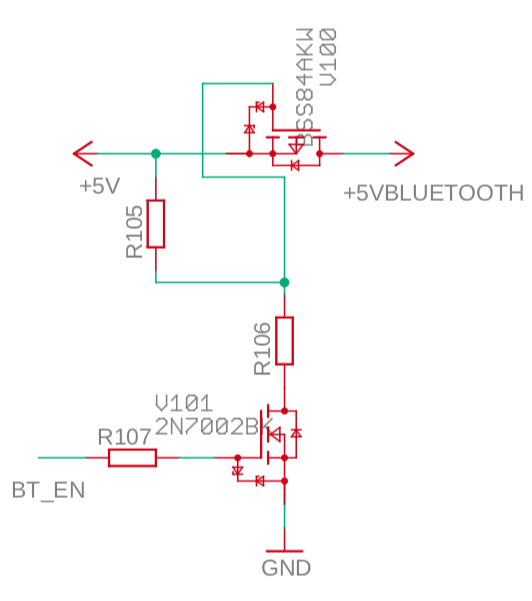
\includegraphics[width=0.7\textwidth]{./img/spannungsabschaltung.png}
  \caption{Spannungsabschaltung 5VBT und 5VGPS}\label{fig.spannungsabschaltung}
\end{figure}

Die Messung des Ladezustands wird über einen einfachen Spannungsteiler realisiert, der so dimensioniert ist, dass maximal 3,37\,V bei vollgeladenem Akku ausgegeben werden. Die genauen Werte sind dem angehängten Stromlaufplan zu entnehmen. Die Ströme werden mittels zweier ACS712 Stromsensoren, die von 5\,V versorgt werden, gemessen und vom Mikrokontroller ausgewertet.

Die Pins des Mikrokontrollers werden über das Powerboard zum im folgenden erläuterten Sensor-Board durchgeschliffen.

\subsection{Sensor-Board}
In Abbildung \ref{fig.sensorboard} wird das finale Layout des Sensor-Boards gezeigt:

\begin{figure}[H]
  \centering
  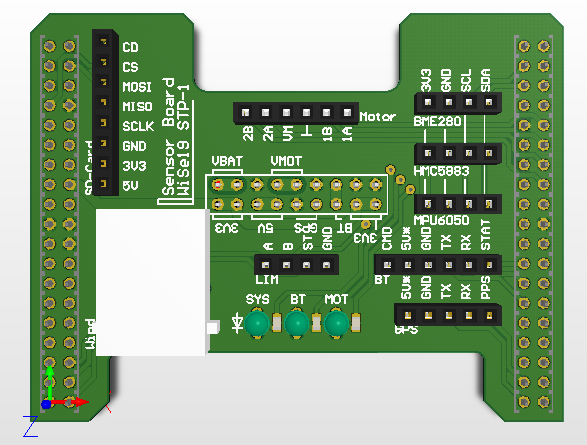
\includegraphics[width=0.7\textwidth]{./img/PCB_Sensors_3D_top.png}
  \caption{Sensor-Board}\label{fig.sensorboard}
\end{figure}

Das Sensor-Board beschränkt sich im Wesentlichen auf die Verdrahtung von Signal- und Spannungsleitungen der Sensoren mit dem Mikrokontroller und den benötigten Spannungen. Die Sensoren werden dabei über Pinheader mit dem Board konnektiert. Drei Status-LEDs, die im späteren Aufbau im Hauptgehäuse nach außen geführt werden, geben Aufschluss über den Status des Systems, Bluetooth-Verbindung und Motoransteuerung.







